% !TEX root = main.tex

\section{事务} % Chap 14
\subsection{基本概念}
\begin{definition}[事务(transaction)]
构成单一逻辑工作单元的操作集合称为事务。
即使有故障,数据库系统也必须保证数据库的正确执行——要么执行整个事务,要么属于该事务的操作一个也不执行。
\end{definition}

事务具有以下的基本性质(ACID):
\begin{itemize}
	\item 原子性(Atomicity):要么执行完,要么不执行,不能执行到一半 $\to$ 日志、恢复系统
	\item 一致性(Consistency):除了基本的数据完整性约束,还有更多的一致性约束。
	\item 隔离性(Isolation):每个事务都察觉不到系统中有其他事务在并发执行,一定是完成一个再进行下一个 $\to$ 并发控制系统
	\item 持久性(Durability):一个事务成功完成对数据库的改变是永久的,即使出现系统故障 $\to$ 结束前已写入磁盘,更新信息已写入磁盘
\end{itemize}

事务的基本状态:
\begin{itemize}
	\item 活动的(active):初始状态
	\item 部分提交的(partially commited):最后一条语句执行后
	\item 失败的(failed):执行出错
	\item 中止的(aborted):事务回滚且数据库已恢复到事务开始执行前
	\item 提交的(commited):成功完成
\end{itemize}
\begin{figure}[H]
\centering
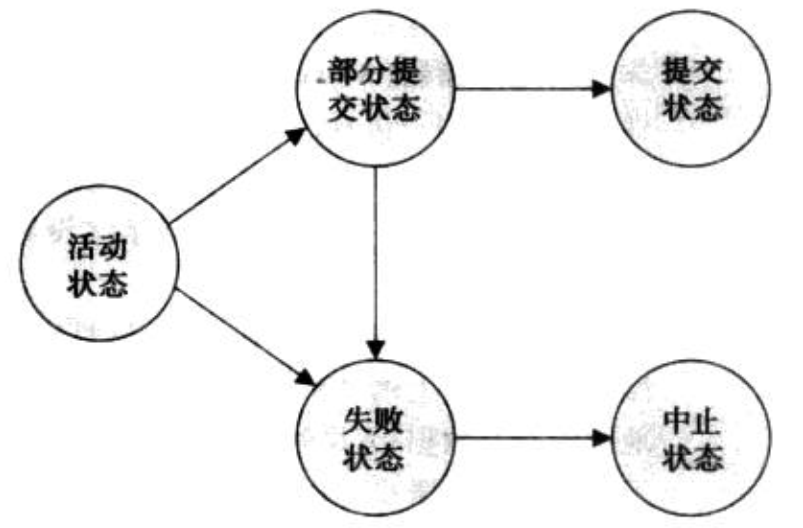
\includegraphics[width=0.3\linewidth]{fig/transaction_state.png}
\end{figure}

\subsection{可串行化}
\begin{definition}[调度]
按照时间顺序执行的一串指令即为调度。
如果事务内的指令都不被打乱,如$<T_1,T_2>$或$<T_2,T_1>$,则为串行调度。
\end{definition}
\begin{definition}[冲突]
当$I$和$J$是不同事务在相同数据项$Q$上的操作,并且其中\textbf{至少有一个}是\verb'write'指令时,则称$I$与$J$是冲突的。
\end{definition}
\begin{definition}[冲突等价(conflict equivalent)]
如果调度$S$可以经过一系列\textbf{非冲突}指令交换转换为$S'$,则称$S$和$S'$是冲突等价的。
若$S'$为串行调度,则$S$为冲突可串行化的(conflict serializable)。
\end{definition}
\begin{figure}[H]
\centering
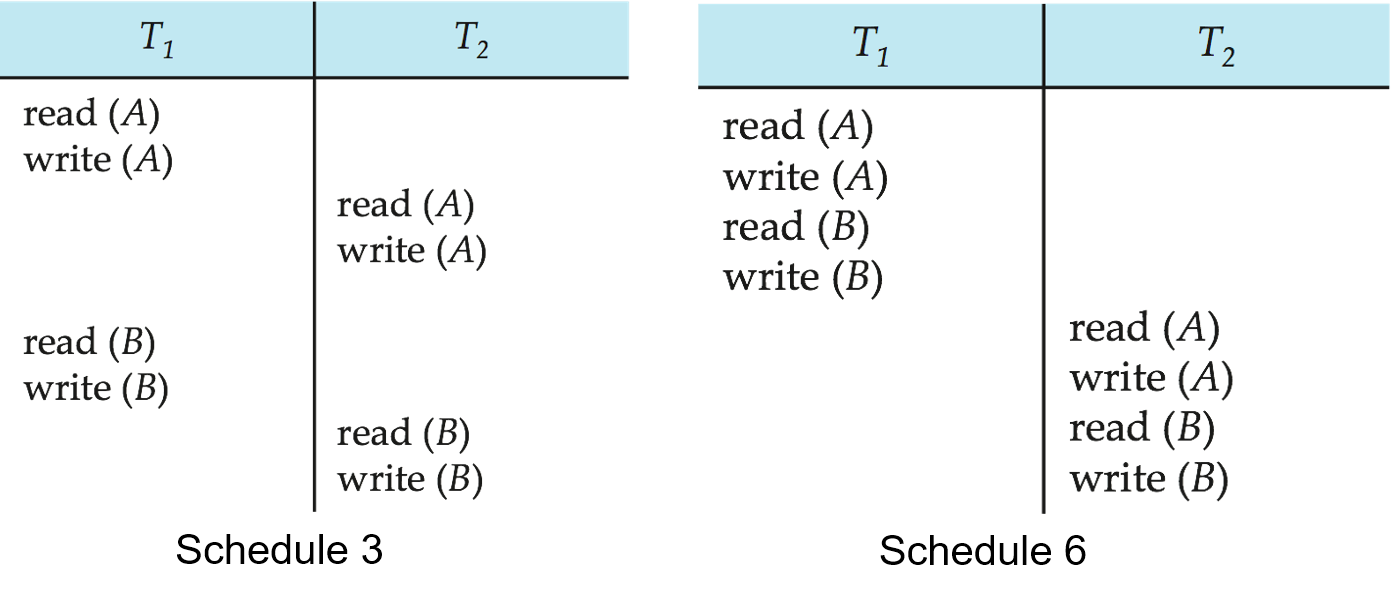
\includegraphics[width=0.8\linewidth]{fig/conflict_serializability.png}
\end{figure}
可以将左侧调度通过两个非冲突指令调换转为右侧,故是冲突可串行的。

可以通过构造一个优先图(precedence graph)来判断是否冲突可串行化,顶点集由所有参与调度的事务构成,边集由满足下列三个条件之一的边$T_i\to T_j$构成:
\begin{itemize}
	\item 在$T_j$执行read(Q)前,$T_i$执行write(Q)
	\item 在$T_j$执行write(Q)前,$T_i$执行read(Q)
	\item 在$T_j$执行write(Q)前,$T_i$执行write(Q)
\end{itemize}
即只有\textemph{两者都读才不冲突,先执行到后执行连边}。

如果无环(用环检测算法),则冲突可串行化,可以通过\textbf{拓扑排序}(所有父亲执行完才到孩子执行)得到串行化顺序。

\begin{definition}[可恢复调度]
若事务$T_j$读事务$T_i$先前写的数据(\textemph{先写后读}),则$T_i$的提交必须在\textemph{$T_j$的提交之前}。
\end{definition}
\begin{definition}[无级联(cascadeless)调度]
若事务$T_j$读事务$T_i$先前写的数据(\textemph{先写后读}),则$T_i$的提交必须在\textemph{$T_j$这一读操作之前}。
\end{definition}

\subsection{隔离性级别}
事务隔离性的好处:提高吞吐量和资源利用率、减少等待时间
\begin{itemize}
	\item 可串行化(serializable)
	\item 可重复读(repeatable read):只允许读已提交数据,一个事务两次读一个数据期间,其他事务不得更新该数据
	\item 已提交读(read committed):只允许读已提交数据,但不要求可重复读
	\item 未提交读(read uncommitted):允许读未提交数据,最低一致性要求
\end{itemize}